% 图 63.5 —— 由 `checks/emit_hand.py` 自动拼出（probe 精测 + prims2 图元分解）
%%
% ⚠ 这是**稿子不是成品**：跑 `checks/checkhand.py 63.5` 看指标 + 看叠合图。
%%
%% ⚠ 待核：
%   · 本图 probe 报出阴影族 1 个 —— **本脚本不生成阴影**（要照原书手写）；prims2 的 strokes 里可能含阴影线，核对时留意别画重
%   · 可疑字形 1 项（空心圈 ⊙ 常被认成字母 o）—— 见文件末
%%
\documentclass[12pt]{standalone}
\usepackage{fontspec}
\setsansfont{Arial}
\newfontfamily\mfallback{DejaVu Sans}
\usepackage{tikz}
\begin{document}
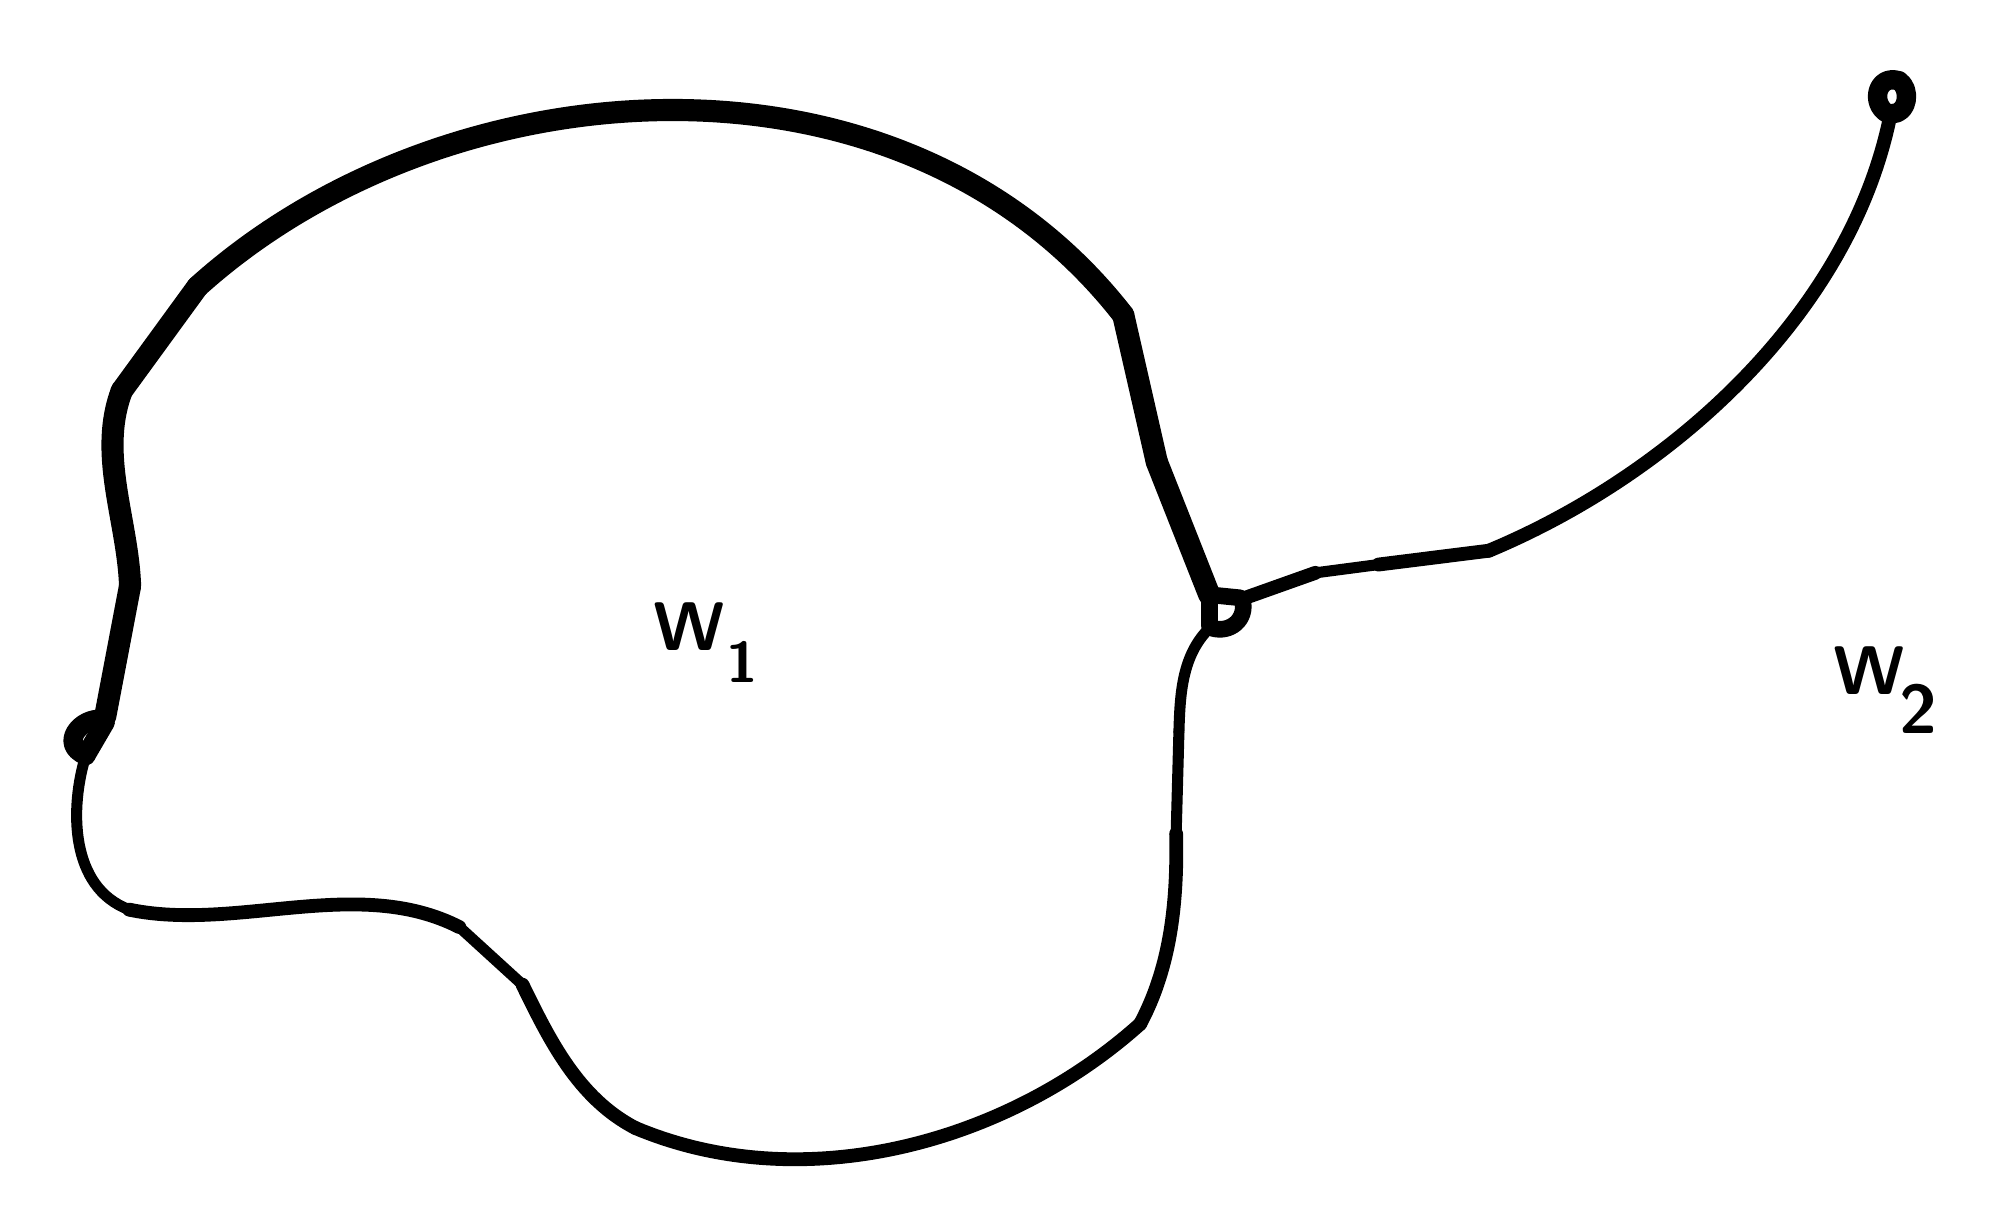
\begin{tikzpicture}[x=1pt, y=-1pt, line width=6.0pt, line cap=round, line join=round]

  %% ════ 直线段（prims2 的 strokes）════
  \draw[line width=6.0pt] (427.0,206.0) -- (427.0,216.0);
  \draw[line width=4.0pt] (416.0,254.5) -- (415.0,291.3);
  \draw[line width=4.0pt] (178.8,345.8) -- (156.0,325.0);
  \draw[line width=8.0pt] (28.0,249.0) -- (37.0,201.7);
  \draw[line width=8.0pt] (34.0,131.2) -- (61.4,93.6);
  \draw[line width=8.0pt] (395.9,103.9) -- (408.0,156.9);
  \draw[line width=8.0pt] (408.0,156.9) -- (427.0,205.0);
  \draw[line width=7.0pt] (21.0,263.0) -- (28.0,251.0);
  \draw[line width=6.0pt] (428.0,205.0) -- (438.0,206.0);
  \draw[line width=5.0pt] (528.0,189.0) -- (488.1,194.0);
  \draw[line width=4.0pt] (488.1,194.0) -- (465.3,197.0);
  \draw[line width=5.0pt] (465.3,197.0) -- (440.0,206.0);

  %% ════ 曲线（prims2 的 curves —— 三段式，坐标同为 (y,x)）════
  \draw[line width=4.0pt] (427.0,217.0) .. controls (417.0,226.9) and (416.4,241.0) .. (416.0,254.5);
  \draw[line width=5.0pt] (415.0,291.3) .. controls (415.5,315.7) and (413.1,339.2) .. (402.0,360.0);
  \draw[line width=5.0pt] (402.0,360.0) .. controls (353.9,403.2) and (280.2,423.1) .. (219.6,397.6);
  \draw[line width=5.0pt] (219.6,397.6) .. controls (198.8,386.8) and (188.5,365.6) .. (178.8,345.8);
  \draw[line width=5.0pt] (156.0,325.0) .. controls (119.2,306.2) and (75.6,326.8) .. (36.7,318.7);
  \draw[line width=4.0pt] (36.7,318.7) .. controls (15.1,310.7) and (15.2,281.7) .. (21.0,263.0);
  \draw[line width=7.0pt] (672.0,31.0) .. controls (665.7,27.4) and (668.2,16.7) .. (676.2,19.2);
  \draw[line width=7.0pt] (676.2,19.2) .. controls (680.6,22.1) and (679.5,31.0) .. (674.0,31.0);
  \draw[line width=8.0pt] (37.0,201.7) .. controls (36.2,178.0) and (25.3,154.2) .. (34.0,131.2);
  \draw[line width=8.0pt] (61.4,93.6) .. controls (151.1,12.7) and (315.8,0.8) .. (395.9,103.9);
  \draw[line width=7.0pt] (21.0,263.0) .. controls (11.0,258.9) and (19.3,248.9) .. (27.0,250.0);
  \draw[line width=5.0pt] (673.0,32.0) .. controls (658.4,103.4) and (594.0,161.5) .. (528.0,189.0);
  \draw[line width=6.0pt] (439.0,207.0) .. controls (440.6,213.8) and (434.6,218.9) .. (428.0,217.0);

  %% ════ 标签（probe 直接给的 \node 行）════
  %% ⚠ 全部补了 fill=white：文字在最上层，否则与曲线交叉干扰
     \node[anchor=center,inner sep=0pt,fill=white,font=\fontsize{28.6}{35.7}\selectfont] at (239.2,216.5) {\textsf{\textbf{\textit{W}}}};   % box(226,205,26,21)
     \node[anchor=center,inner sep=0pt,fill=white,font=\fontsize{22.2}{27.8}\selectfont] at (258.1,229.4) {\textsf{\textbf{1}}};   % box(252,221,7,16)
     \node[anchor=center,inner sep=0pt,fill=white,font=\fontsize{28.0}{35.0}\selectfont] at (665.7,232.4) {\textsf{\textbf{\textit{W}}}};   % box(653,221,25,21)
     \node[anchor=center,inner sep=0pt,fill=white,font=\fontsize{22.9}{28.7}\selectfont] at (683.1,246.4) {\textsf{\textbf{2}}};   % box(677,238,11,16)

  % 钉死画布：否则超出的图元/控制点会把页面撑大，1:1 回比就失准
  \pgfresetboundingbox
  \path[use as bounding box] (0,0) rectangle (699,421);
\end{tikzpicture}
\end{document}

% ⚠ 待核清单（probe 拿不准，人眼过一遍）：
%   · 未识别/跳过：⑤ 跳过/未识别的字形
